\documentclass[12pt, letterpaper]{article}

% --- Packages ---
\usepackage{geometry}
 \geometry{margin=1in}
\usepackage{graphicx}
\usepackage{amsmath, amssymb}
\usepackage{booktabs}
\usepackage{hyperref}
\usepackage{cite}
\usepackage{setspace}
\onehalfspacing
\usepackage{fontspec}
\usepackage{polyglossia}
\usepackage{float}
\usepackage{svg}
\usepackage{enumitem}
\setmainlanguage{vietnamese}

\usepackage{listings}
\usepackage{xcolor}

\lstset{
    language=C,
    basicstyle=\ttfamily\small,
    keywordstyle=\color{blue},
    stringstyle=\color{red},
    commentstyle=\color{green!60!black},
    breaklines=true,
    frame=single, % Tạo khung xung quanh code
    backgroundcolor=\color{gray!5}
}

\renewcommand{\lstlistingname}{Mã nguồn}

% --- Metadata ---
\title{Giải bài tập 13}
\author{Đỗ Hoàng Gia Bảo - 23020783 \\ \small Khoa Điện tử - Viễn Thông}
\date{\today}

\begin{document}

\maketitle

\begin{abstract}
Báo cáo sẽ trình bày phần làm bài tập slide 43, Bài-7
\end{abstract}
% --- Front Matter (Roman Numerals) ---
\newpage
\tableofcontents

% --- Main Content (Arabic Numerals) ---
\newpage
\pagenumbering{arabic}
\setcounter{page}{3} % This automatically resets the counter to 1

\section{Bài tập}
Hệ điều hành có 256 KB bộ nhớ trong, ban đầu trống hoàn
toàn. Các tiến trình yêu cầu sử dụng bộ nhớ với kích thước
5 KB, 25 KB, 35 KB, 20 KB.
\begin{itemize}
    \item Hãy mô tả cách hệ thống Buddy đáp ứng mỗi yêu cầu, vẽ sơ đồ bộ
nhớ tương ứng.
    \item Sau khi cấp phát hết các yêu cầu trên, hệ thống sẽ làm gì nếu tiến
trình với yêu cầu bộ nhớ 25 KB kết thúc và giải phóng bộ nhớ ?
\end{itemize}
\section{Giải bài tập}
\subsection{Ý thứ nhất}
\textbf{Cách hoạt động của hệ thống Buddy}

Khi nhận một yêu cầu, bộ nhớ được chia đôi đệ quy đến khi kích thước của một khối nhớ vừa đủ để lưu yêu cầu.

\noindent \textbf{Sơ đồ bộ nhớ}


Hệ thống sẽ đáp ứng các yêu cầu như bảng dưới đây:
\begin{figure}[H]
    \centering
    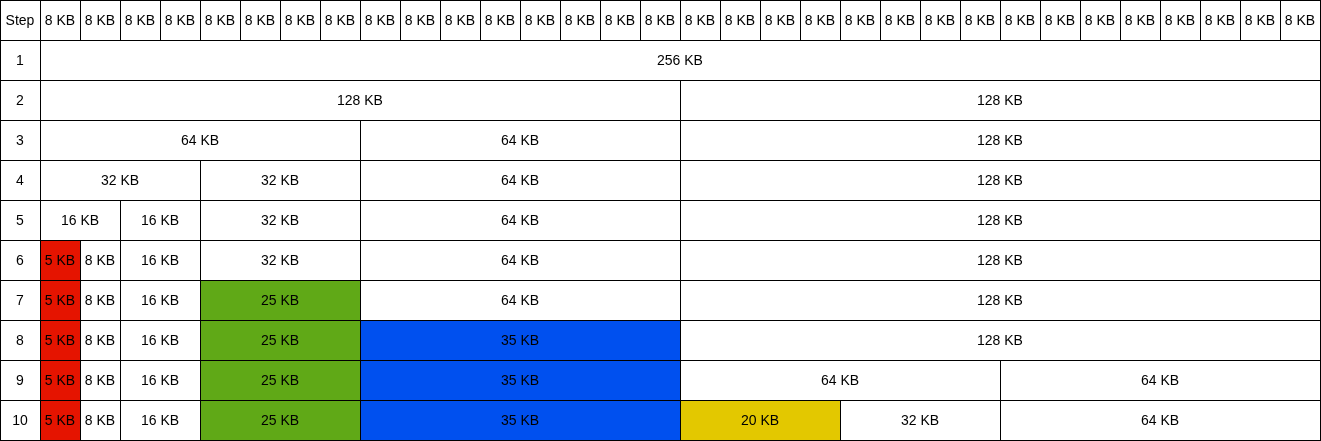
\includegraphics[width=1.0\textwidth]{Images/memory_states.png}
    \caption{Bảng trạng thái của bộ nhớ trong sử dụng hệ thống Buddy}
\end{figure}
\begin{enumerate}
    \item Kiểm tra tiến trình (5 KB): 256 KB $>>$ 5 KB $\rightarrow$ Chia khối nhớ làm đôi và chọn khối nhớ có chỉ số thấp hơn (khối nhớ bên trái).
    \item Kiểm tra tiến trình (5 KB): 128 KB $>>$ 5 KB $\rightarrow$ Chia khối nhớ làm đôi và chọn khối nhớ có chỉ số thấp hơn (khối nhớ bên trái).
    \item Kiểm tra tiến trình (5 KB): 64 KB $>>$ 5 KB $\rightarrow$ Chia khối nhớ làm đôi và chọn khối nhớ có chỉ số thấp hơn (khối nhớ bên trái).
    \item Kiểm tra tiến trình (5 KB): 32 KB $>>$ 5 KB $\rightarrow$ Chia khối nhớ làm đôi và chọn khối nhớ có chỉ số thấp hơn (khối nhớ bên trái).
    \item Kiểm tra tiến trình (5 KB): 16 KB $>>$ 5 KB $\rightarrow$ Chia khối nhớ làm đôi và chọn khối nhớ có chỉ số thấp hơn (khối nhớ bên trái).
    \item Kiểm tra tiến trình (5 KB): 8 KB $>$ 5 KB $\rightarrow$ Yêu cầu được lưu vào khối nhớ 8 KB có chỉ số thấp hơn (khối nhớ bên trái).
    \item Kiểm tra tiến trình (25 KB): Hệ thống sử dụng khối 32 KB đang trống sẵn từ chia tách trước đó để cấp phát (Khối nhớ 32 KB bên phải).
    \item Kiểm tra tiến trình (35 KB): Hệ thống sử dụng khối 64 KB đang trống sẵn từ chia tách trước đó để cấp phát (Khối nhớ 64 KB bên phải).
    \item Kiểm tra tiến trình (20 KB): Vì khối bộ nhớ ở 128 KB ở bên trái đã được chia cắt và sử dụng bởi các yêu cầu tiến trình trước nên phải chia đôi khối 128 KB ở bên phải. 128 KB $>>$ 20 KB $\rightarrow$ Chia khối nhớ làm đôi và chọn khối nhớ có chỉ số thấp hơn (khối nhớ bên trái).
    \item Kiểm tra tiến trình (5 KB): 64 KB $>>$ 20 KB $\rightarrow$ Chia khối nhớ làm đôi và chọn khối nhớ có chỉ số thấp hơn (khối nhớ bên trái).
    \item Kiểm tra tiến trình (20 KB): 32 KB $>$ 20 KB $\rightarrow$ Yêu cầu được lưu vào khối nhớ 32 KB có chỉ số thấp hơn (khối nhớ bên trái).
\end{enumerate}
\subsection{Ý thứ hai}
Khí tiến trình với yêu cầu bộ nhớ 25 KB kết thúc và giải phóng bộ nhớ, hệ thống Buddy sẽ cập nhật trạng thái bộ nhớ như bảng dưới đây:
\begin{figure}[H]
    \centering
    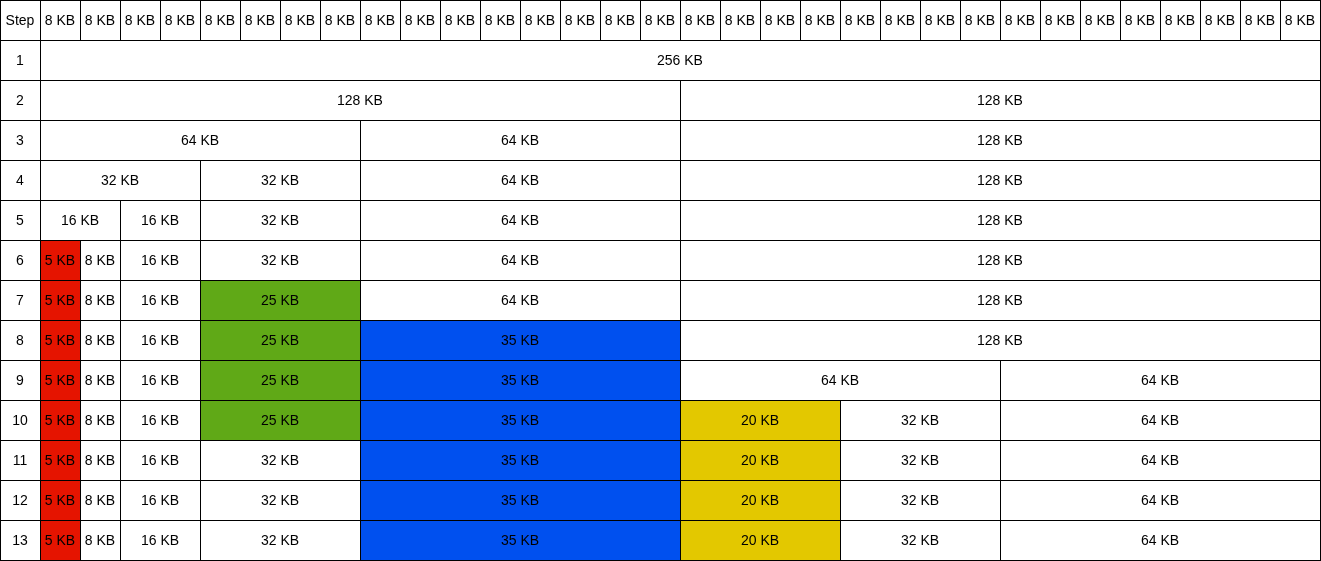
\includegraphics[width=1.0\textwidth]{Images/new_memory_state.png}
    \caption{Bảng trạng thái của bộ nhớ trong sau khi giải phóng bộ nhớ tiến trình với yêu cầu bộ nhớ 25 KB}
\end{figure}
Cụm bên trái này không hoàn toàn trống vì nhánh con của nó đang chứa P1 (5 KB). Do đó, khối buddy 32 KB bên trái được tính là đang bận. Vì khối buddy đối xứng của nó không trống, hệ thống không thể tiến hành gộp khối 32 KB này lên thành khối 64 KB được. 
\end{document}